% Tabela: Configurações descartadas no experimento Gamma
\begin{table}[H]
	\centering
	\caption{Configurações descartadas de análises pelo Experimento 2.}
	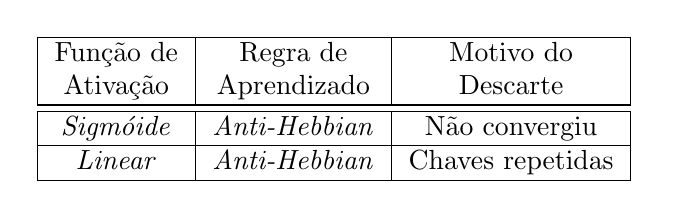
\begin{tikzpicture}

		\node[thick, align=center] (table) {
			\begin{tabular}{ |c|c|c| }
				\hline
				% \multicolumn{3}{ |c| }{Configurações descartadas nas análises} \\
				% \hline \hline
				Função de & Regra de & Motivo do\\
				Ativação & Aprendizado & Descarte\\
				\hline \hline
				\textit{Sigmóide} & \textit{Anti-Hebbian} & Não convergiu   \\ \hline
				\textit{Linear} & \textit{Anti-Hebbian} & Chaves repetidas  \\ \hline
			\end{tabular}
		};

	\end{tikzpicture}
% 	\caption{Configurações descartadas de análises pelo Experimento 2.}
	\label{tab:configuracoesDescartadasGamma}
\end{table}